%\addcontentsline{toc}{chapter}{Development Process}
\chapter{Design \& Implementation}

The structure of this chapter follows the agile methodology used to develop the
Quiz Tool. Each section contains information about a sprint, allowing the reader
to gain more understanding of how the design and the tool itself evolved over time.

\section{Sprint 1 - Hello Quiz Tool}
\subsection{Sprint Planning}
The first sprint of the Quiz Tool focused on setting up the DevOps of the project,
and deployment of a "hello world" version of the tool consisting of the front end,
back end and nginx\cite{34} running together using docker-compose. It was also important
to investigate how to best structure the application to include both the front and the
back end of the application in a single GitHub repository. The following subsections
cover the most important aspects of the sprint, and the entire list of estimated
stories can be found in the \autoref{chap:spintstories} of this report.

\subsection{Application Structure}
The main goal of using docker-compose, was to have the whole application running in
the same manner locally on the developer's machine, during testing on Circle CI, and
in the production environment. This meant the application had to be containerised
using Docker, and containers had to be able to communicate with each other appropriately.
This was even more difficult considering Socket.io had to be incorporated, to allow
real time broadcast of lecture slides to students in the future. I have decided to
create a prototype of a very basic chat application, containerised using Docker and
orchestrated using docker-compose. The prototype had to be written in the MEAN stack,
and use Socket.io to prove it was possible to make all technologies work together.

\begin{figure}[ht]
    \centering
    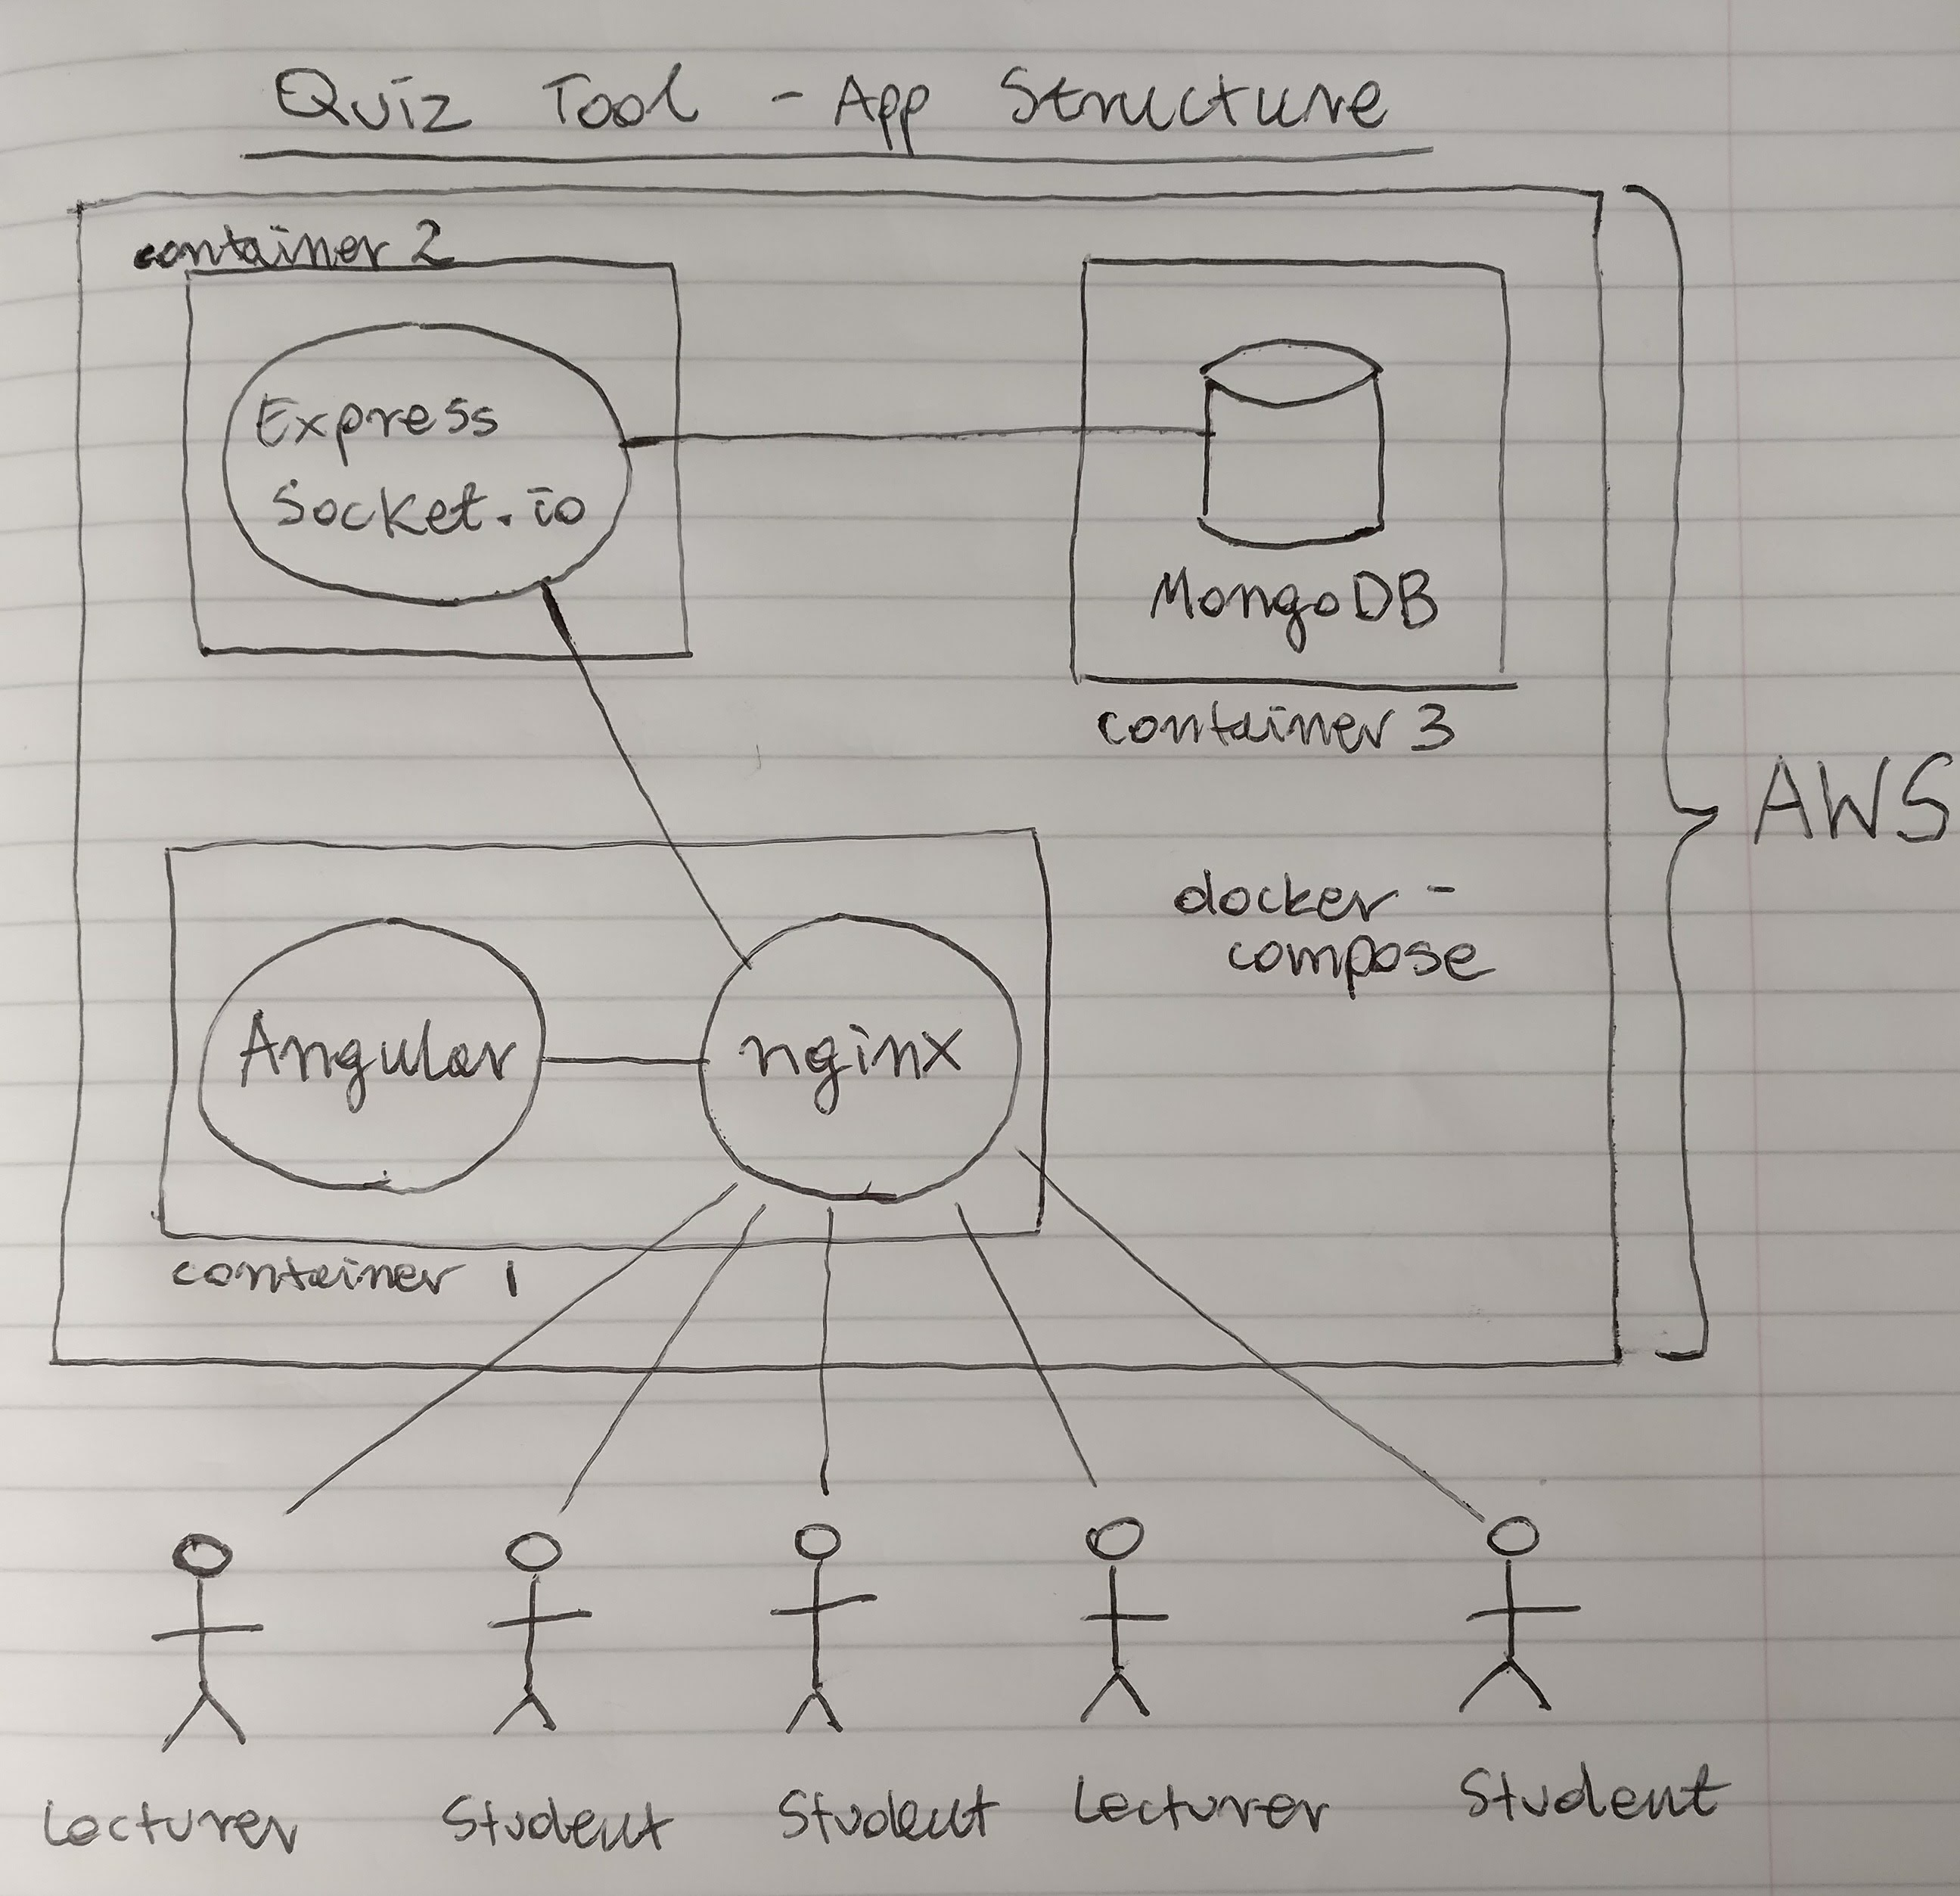
\includegraphics[width=0.7\textwidth]{../../design/app_structure.jpg}
    \caption{The proof of concept application structure}
    \label{fig:appstrucure}
\end{figure}

\begin{figure}[h!]
  \begin{lstlisting}[basicstyle=\small]
  version: '2.0'
  services:
    client:
      build: client
      ports:
        - "80:80"
      links:
        - server_node
    server_node:
      build: server
      links:
        - database
    database:
      image: mongo
      ports:
        - "27017:27017"
  \end{lstlisting}
  \caption{The docker-compose.yml file describing the tool's structure}
\end{figure}

\newpage
\subsubsection{Front End Container}
The front end container consisted of Angular 4 and nginx reverse proxy. The structure
has been based on the \textit{Dockerized Angular 4 App (with Angular CLI)} repository\cite{35}.
The Socket.io client dependency has been added to allow sending messages to the back end
using sockets. The initial \texttt{Dockerfile} included in the \autoref{chap:codesamples} of this report
as the \autoref{sample:clientdocker} uses the multi-stage build added in Docker 17.05. The
Angular app is compiled to JavaScript and HTML files during the initial stage of the build,
and then these files are copied to the nginx public folder to be served to clients.
This results in a lean, production ready image.

\subsubsection{Back End Container}
The back end container included in the \autoref{chap:codesamples} of this report
as the \autoref{sample:serverdocker} consisted of a Node.js runtime, the Express framework and the Socket.io
engine capable of pushing messages to clients using Sockets. The \texttt{Dockerfile} illustrates
the very basic Node container.

\subsubsection{Database Container}
Finally, the MongoDB Docker image has been pulled automatically from the official mongo
Docker Hub registry\cite{36}.

\subsection{Continuous Integration}
Circle CI has been integrated with the GitHub repository containing the source code of the
Quiz Tool. Every time a pull request was made, Circle CI would be notified. It would then
assign a virtual machine build agent from a pool, and spin up a clean build environment.
It would then checkout the code and run the steps specified in the build config file, before
reporting if the build was successfull back to GitHub.

\begin{figure}[ht]
    \centering
    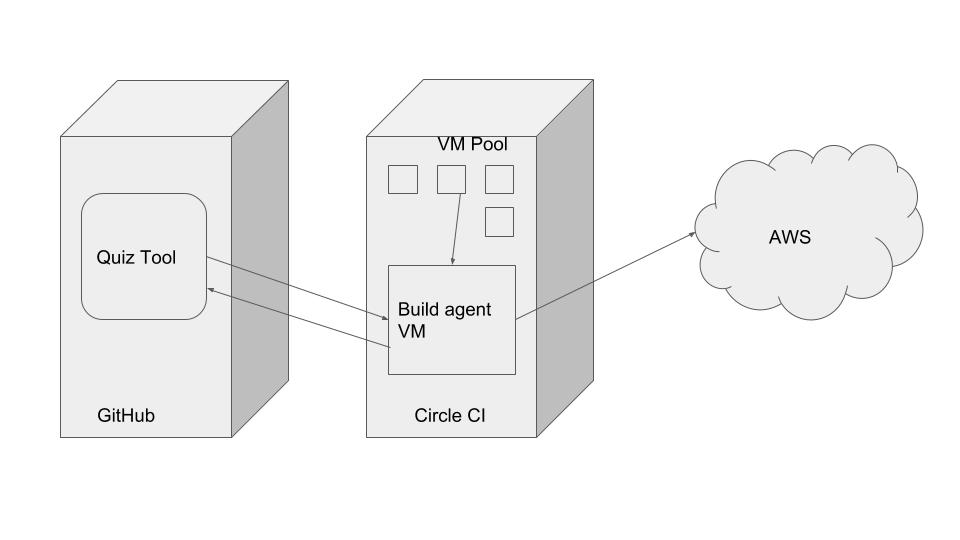
\includegraphics[width=0.8\textwidth]{circleci.jpg}
    \caption{Continuous Integration and Deployment}
    \label{fig:ci}
\end{figure}

The \texttt{.circleci/config.yml} file included in the \autoref{chap:codesamples} of this report
as the \autoref{sample:circleci}, describes the initial build steps of the Quiz Tool.
Code is checked out from the version control, all the dependencies necessary to perform following
steps are installed, the project is then built and started using docker-compose, before the
\texttt{curl localhost} command checks if the application is up and running. Finally, if
the current branch being built is \texttt{master}, the \texttt{deploy.sh} bash script runs, which
deploys the application to production.

\subsection{Production Environment}
The production environment of the tool is hosted on the AWS cloud. The AWS Elastic Beanstalk
has been chosen specificaly, as applications in
various programming languages can be deployed with ease, wihout having to worry about
the infrastructure running these applications\cite{37}. The Multicontainer Docker AWS Elastic
Beanstalk\cite{38} environment, creates a single Amazon EC2\cite{39}
instance and uses ECS (Amazon Elastic Container Service)\cite{40} to coordinate container deployments to
multicontainer Docker environments. The similarity with docker-compose, means the Quiz Tool
would behave similarly on developer's machine, in testing and in production.

\begin{figure}[h!]
    \centering
    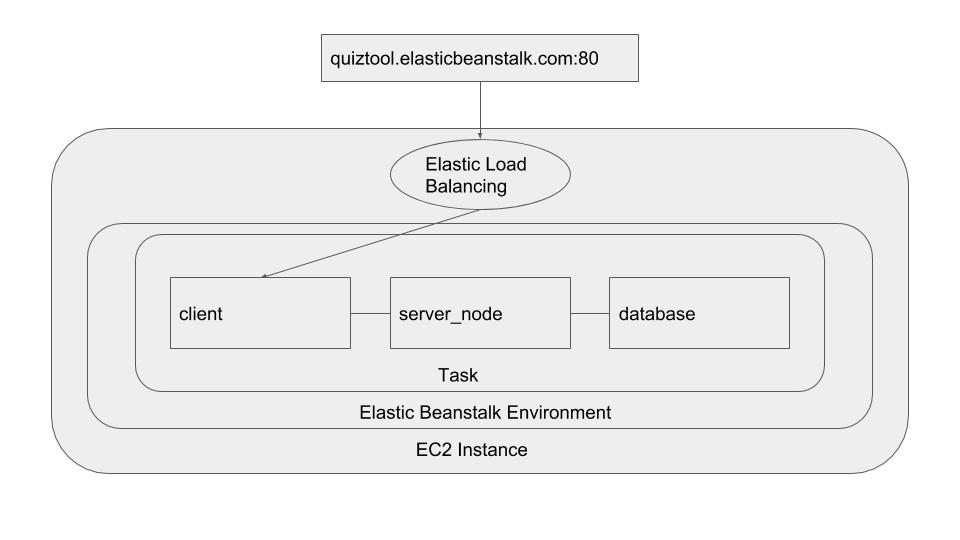
\includegraphics[width=0.8\textwidth]{elasticbeanstalk.jpg}
    \caption{Quiz Tool Production Environment}
    \label{fig:ebs}
\end{figure}

\texttt{docker-compose.yml} files define how docker-compose should run Docker containers together.
\texttt{Dockerrun.aws.json} is the equivalent configuration file to specify relationships between Docker
containers running in the Multicontainer Elastic Beanstalk environment. The format of the config file
included in the \autoref{chap:codesamples} of this report
as the \autoref{sample:dockerrunaws} is very
similar to the docker-compose configuration files. The major
difference is that the AWS Elastic Beanstalk does not build Docker images itself, and images have
to be pulled dynamically from Docker registries. Docker registries are simply servers used for storage and
distribution of Docker images.

\subsubsection{Circle CI and AWS Integration}
The build agent automatically deploys the tool to production when the \texttt{master}
branch is being built. The bash script included in the \autoref{chap:codesamples} of this report
as the \autoref{sample:deploy} performs the actual deployment, and the
approach is based on the examples\cite{41}\cite{42}.
The \texttt{\$AWS\_ACCESS\_KEY\_ID} and the \texttt{\$AWS\_SECRET\_ACCESS\_KEY} environment
variables have been added to the build configuration using the Circle CI web panel.
The integration has been achieved by creating an AWS profile config file and installing
the \texttt{awsebcli} Elastic Beanstalk command line utility as one of the build steps.
Both \texttt{client} and \texttt{server\_node} containers are then tagged and pushed
to the private Docker image registry provided by Amazon Elastic Container Service, before
the \texttt{eb deploy prod-env} command actually triggers the production deployment.
Both front and back end containers are then pulled from the private registry specified
in the \texttt{Dockerrun.aws.json} file, while the mongo image is pulled directly from
the official mongo Docker hub.

\begin{figure}[h!]
    \centering
    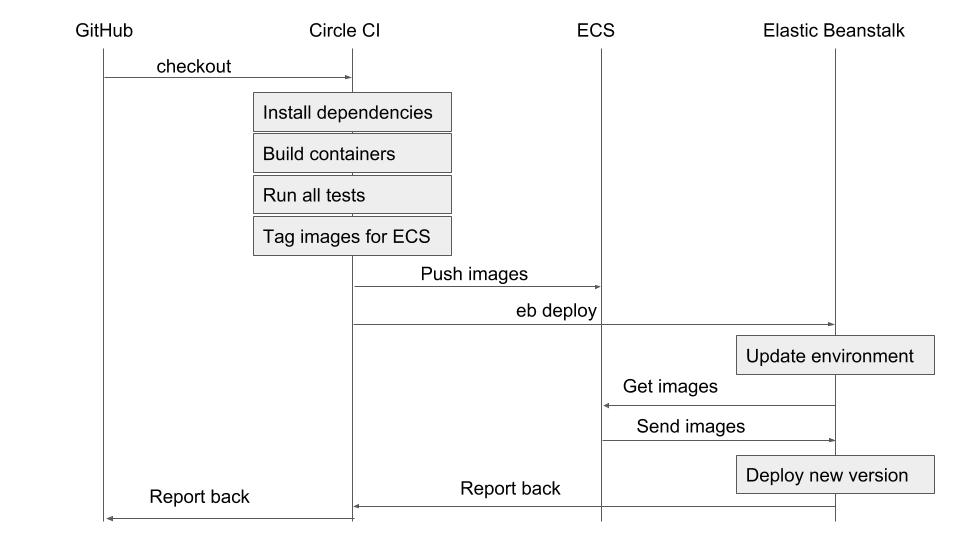
\includegraphics[width=0.8\textwidth]{deployment.jpg}
    \caption{Production Deployment Visualised}
    \label{fig:deploymentprocess}
\end{figure}

\subsection{Story Boards}
Including the customer
early in the development and design process allows teams to stay on track and readjust
their design if necessary. The story boards below have been produced to gain feedback
from the client, and ease the front end development in future iterations.

\autoref{fig:storylecturer} shows how the lectuer would login into the tool using
Google Single Sign On. He could then upload his lecture slides using an action
button in the bottom right corner of the screen, be able to edit his slides and
mark certain slides as quizzes. A list of cards would be presented showing all
lectures belonging to the lecturer and he could broadcast them to his audience.
Subsequently, he could navigate through the slides and slides with embedded quizzes would
split the screen in half to show a bar chart with answers as they come in. Finally,
lecture would end once he clicks the end button.

\autoref{fig:storystudent} on the other hand, shows how students could interact with
the tool. Student could join an ongoing lecture using a session key provided by the
lecturer. She could then participate in the lecture by watching the slides, and
submitting answers to quizzes as they come in. The correct answer could be presented
back to her in a form of a bar chart.

\begin{figure}[h!]
    \centering
    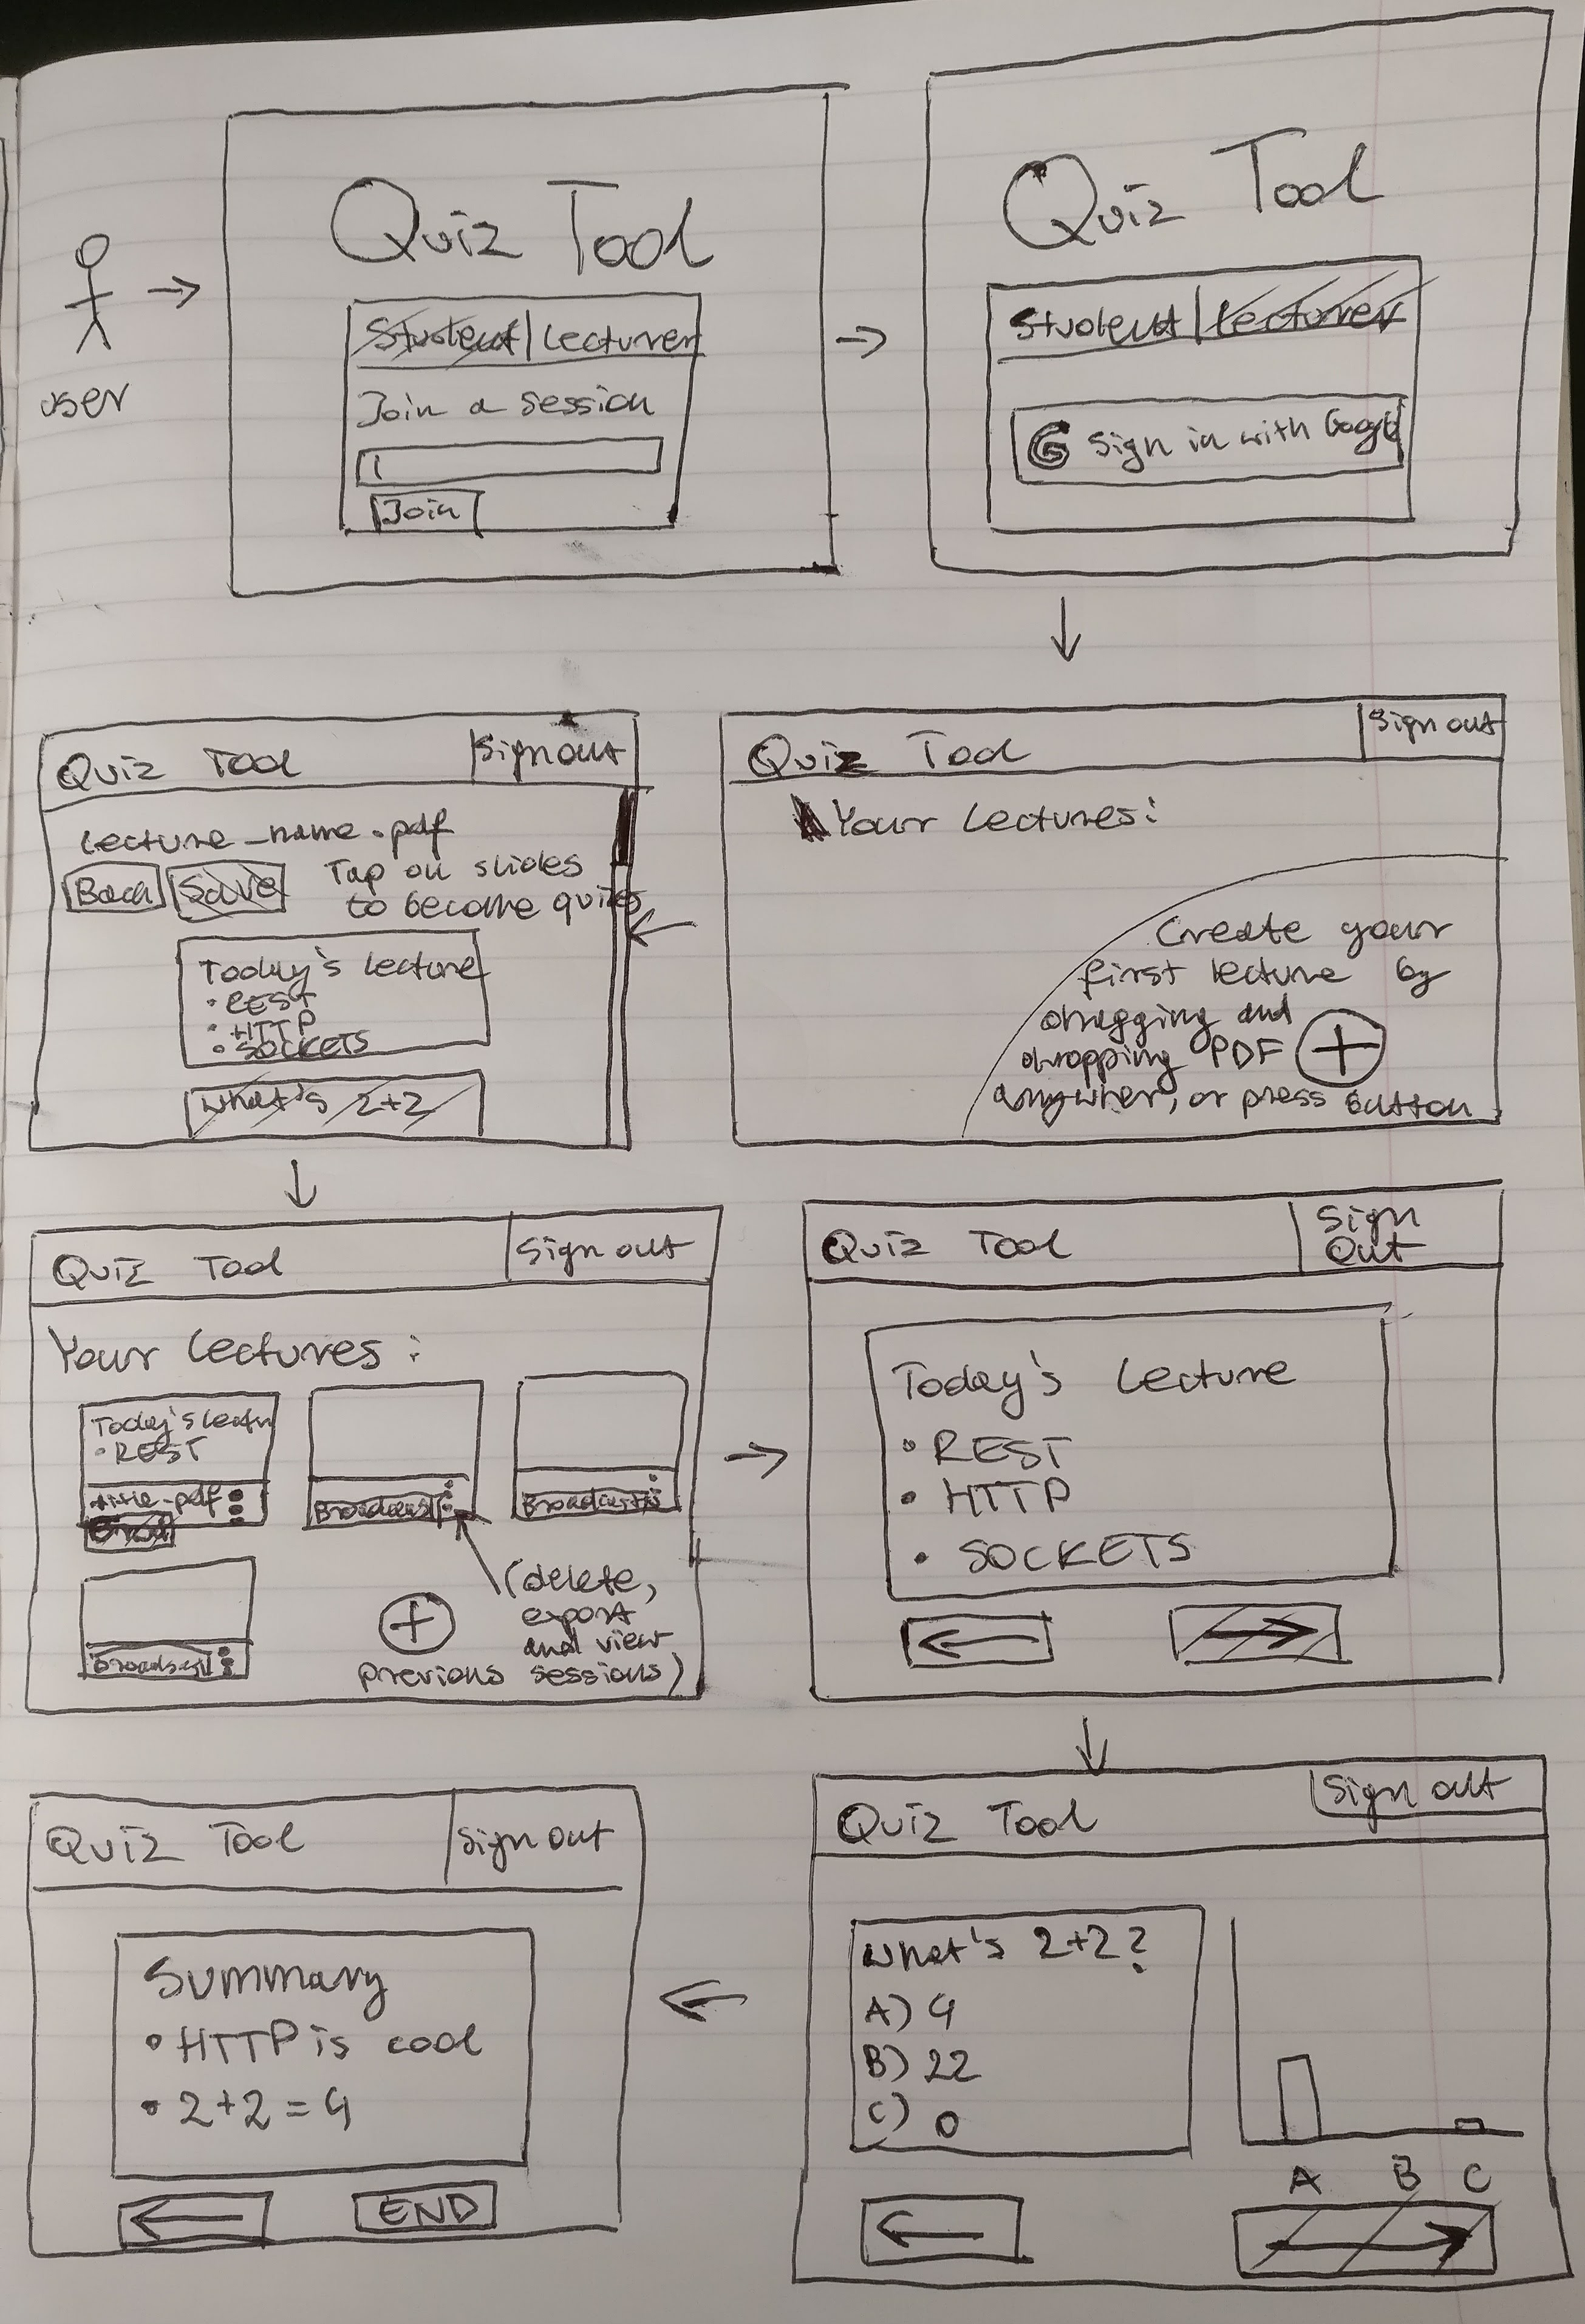
\includegraphics[width=0.9\textwidth]{../../design/story_board_lecturer.jpg}
    \caption{Story Board Lecturer Interaction}
    \label{fig:storylecturer}
\end{figure}

\begin{figure}[ht]
    \centering
    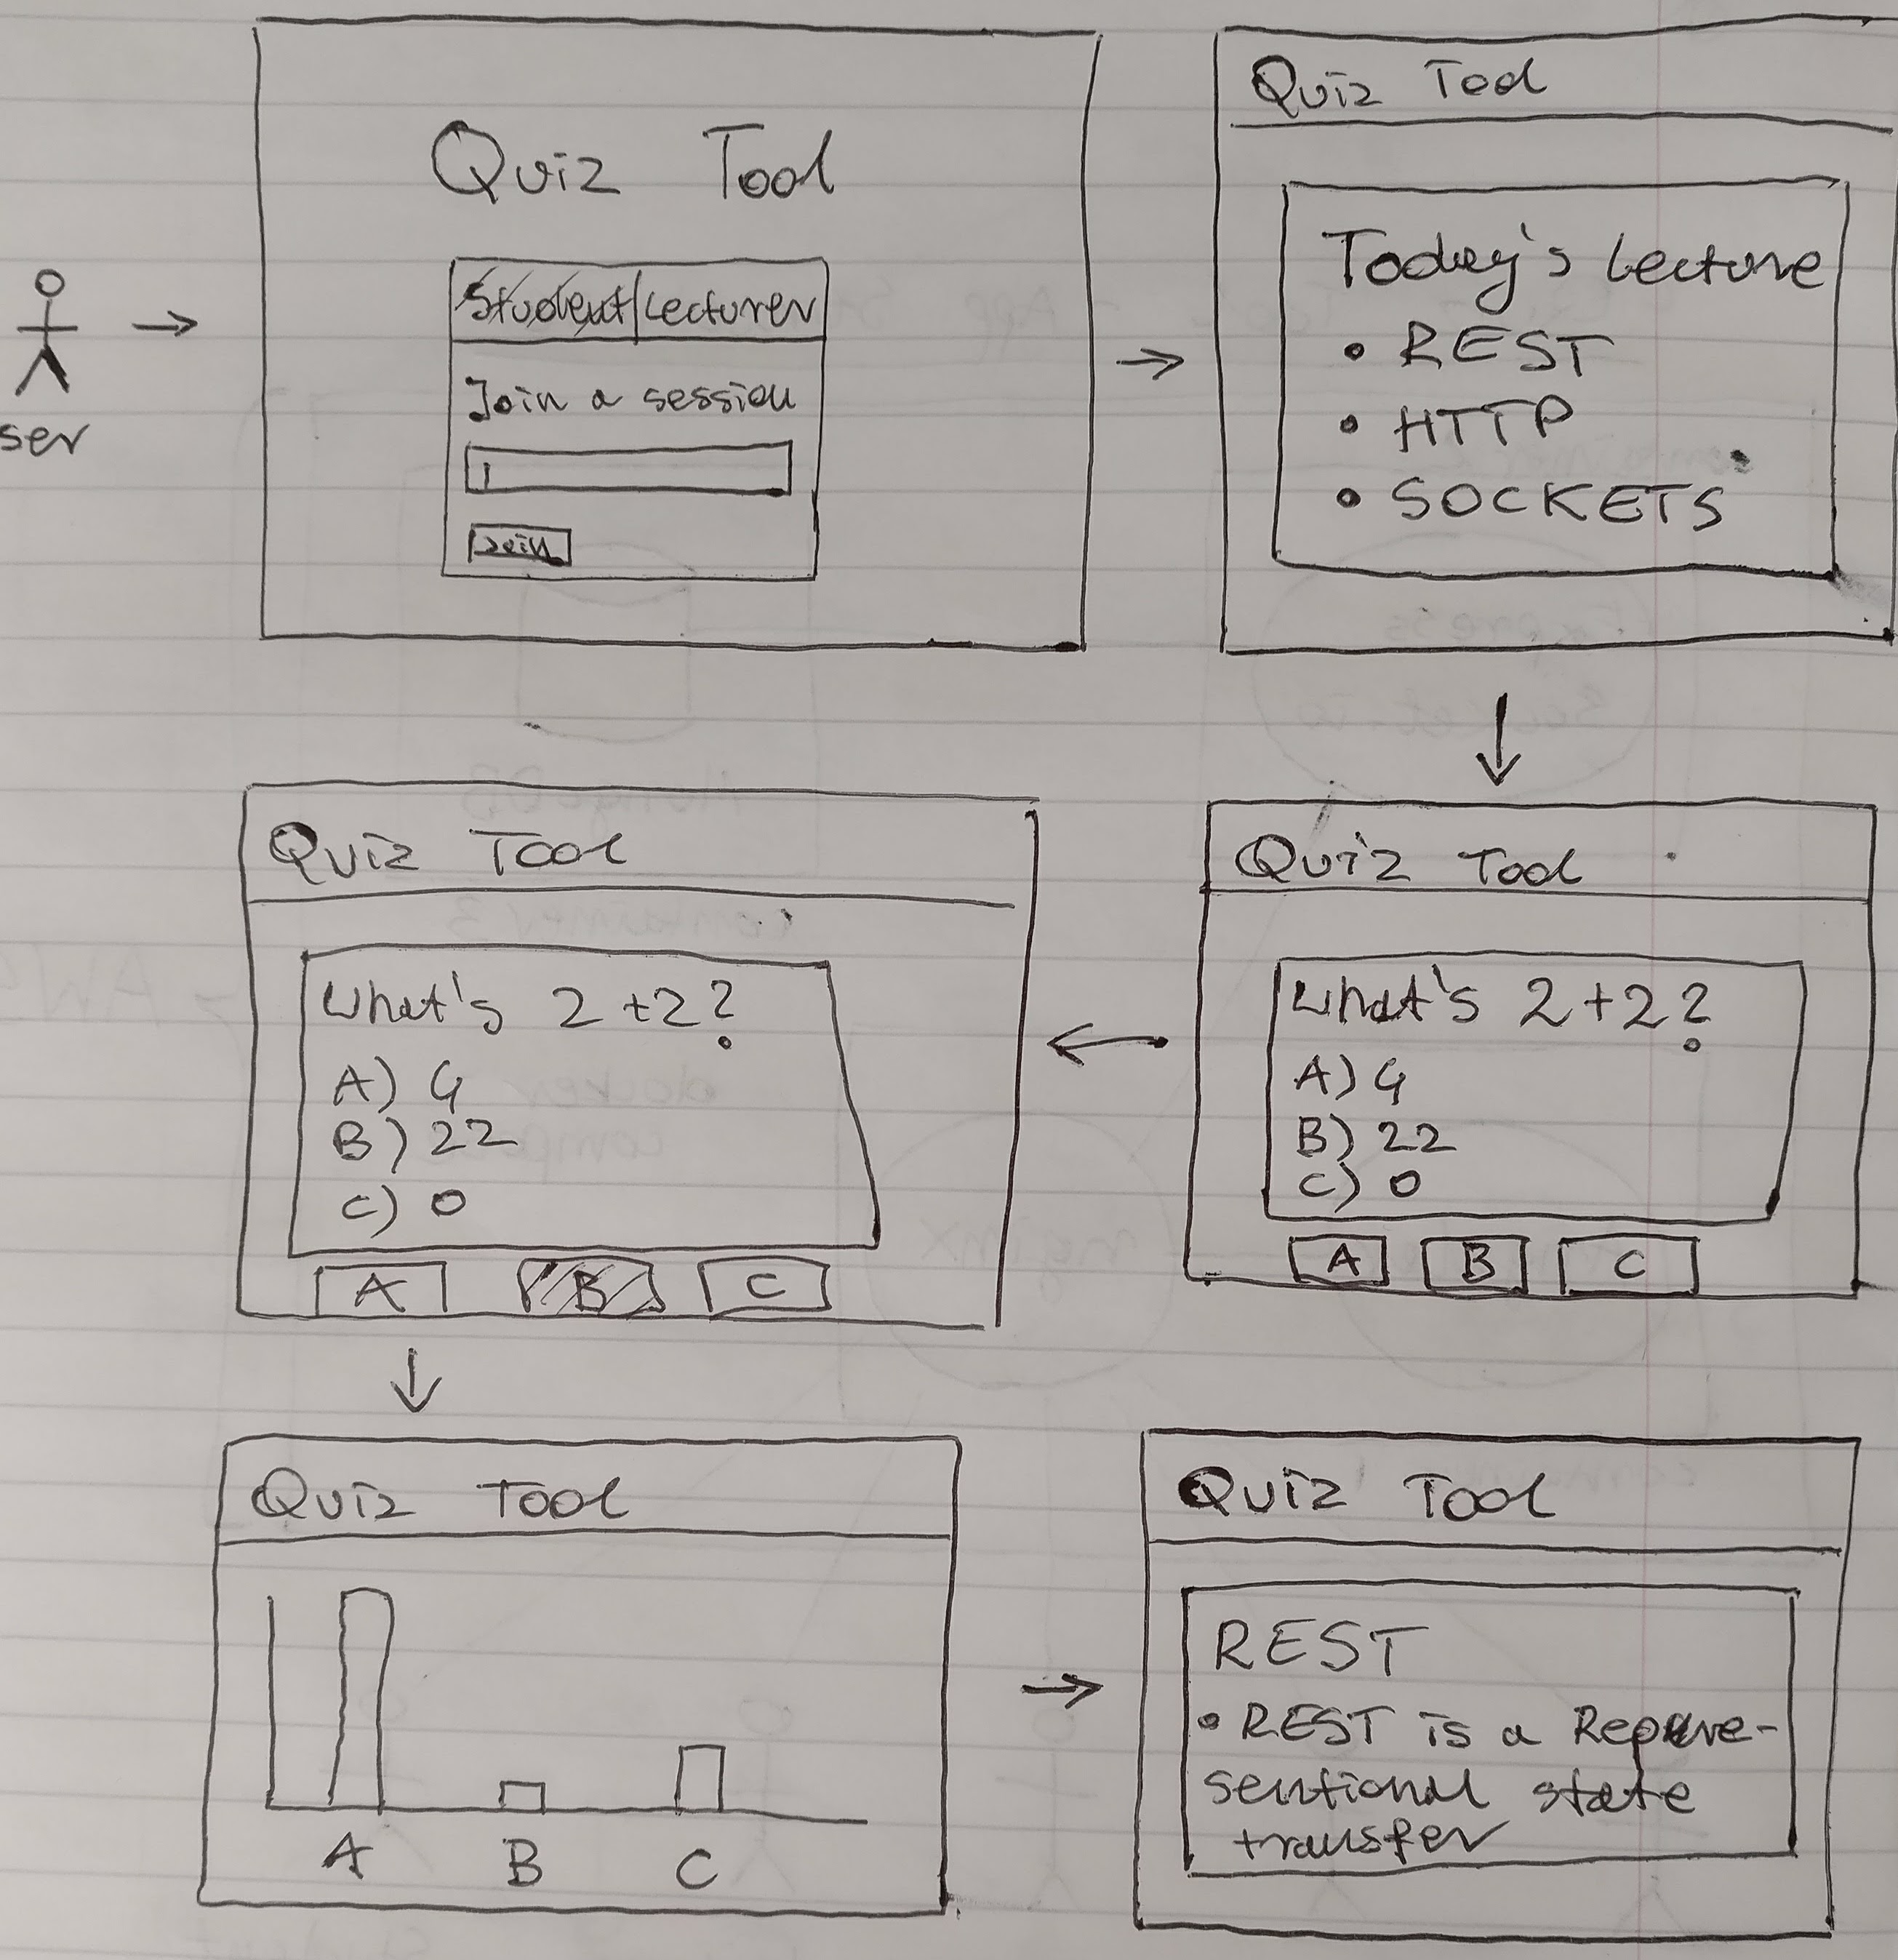
\includegraphics[width=0.9\textwidth]{../../design/story_board_student.jpg}
    \caption{Story Board Student Interaction}
    \label{fig:storystudent}
\end{figure}

\newpage
\subsection{Sprint Retrospective}
The first sprint proved it was possible to deploy a MEAN stack, containerised application
to production using Circle CI. Crucial DevOps has been successfully put in place, and the
initial feedback has been gathered from the client thanks to the low fidelity prototypes.
The full sprint retrospective document produced can be found in the \autoref{chap:spintretrospectives} of this report.

\begin{figure}[ht]
    \centering
    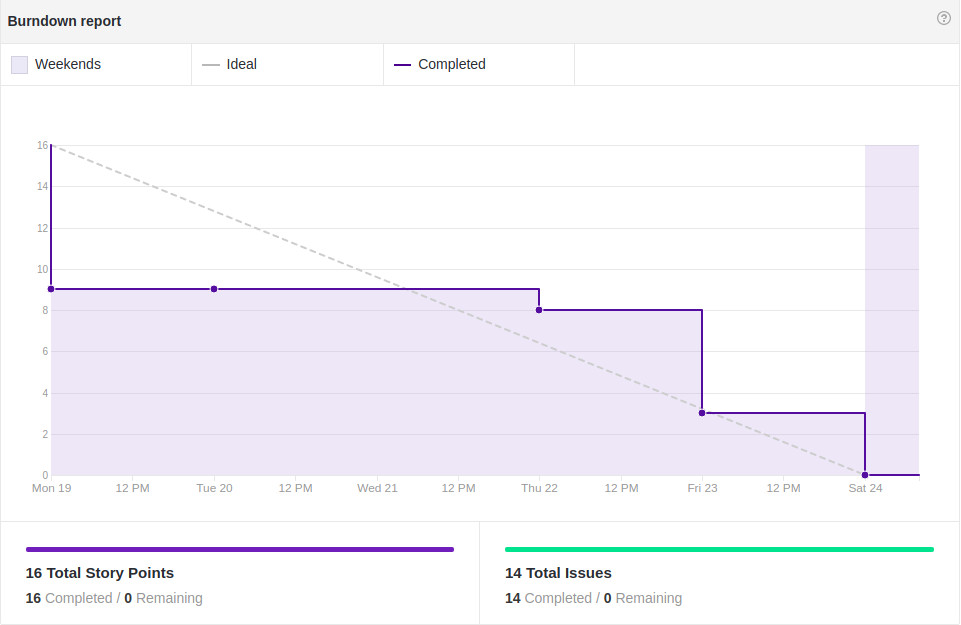
\includegraphics[width=\textwidth]{burn1.jpg}
    \caption{Burndown Chart Sprint 1}
    \label{fig:burn1}
\end{figure}

\newpage
\section{Sprint 2 - Bare Bone Application}
\subsection{Sprint Planning}
This sprint focused on converting the proof of concept chat application created in the previous
week into a basic Quiz Tool. Simple login page for both students and lectuers
would be developed based on the paper prototypes from the previous sprint, and Google Single Sign
On would be added. Once logged in, lectuers could upload their PDF lecture slides and broadcast
them to all students, as session generation was not implemented yet. The entire list of estimated stories
can be found in the \autoref{chap:spintstories} of this report.

\newpage
\subsection{Login Page and Authorisation}
% - JWT tokens
% - JWT interceptor
% - Google single sign on
% - session cookies
The login page has been created based on the low fidelity prototypes, and allowed
lecturers to log into the tool, and students to join ongoing lectures with a session key.
The Materialize\cite{43} CSS framework has been added to achieve a modern user interface.

\begin{figure}[h!]
    \centering
    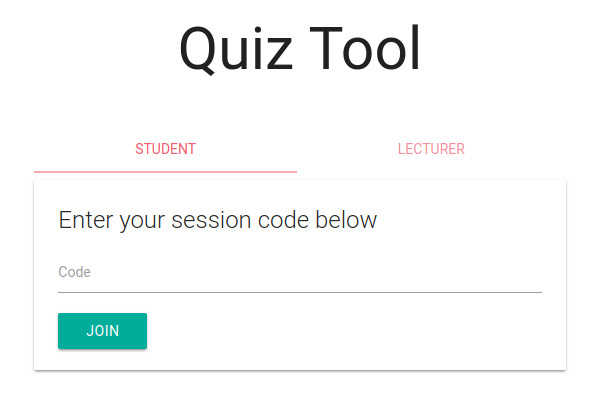
\includegraphics[width=0.8\textwidth]{student_login.jpg}
    \caption{Student Login Page}
    \label{fig:studentlogin}
\end{figure}

\begin{figure}[h!]
    \centering
    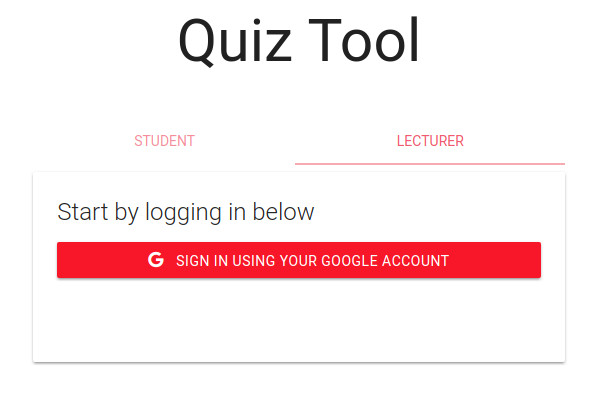
\includegraphics[width=0.8\textwidth]{lecturer_login.jpg}
    \caption{Lecturer Login Page}
    \label{fig:lecturerlogin}
\end{figure}

Angular has a concept of guards, which allow specified routes to be only accessible to
authorised users. The code extracted from the \texttt{client/src/app/app.routing.ts} below
shows how the desired behaviour has been achieved. All undefined routes redirect to the \texttt{/}
which has a \texttt{canActivate: [AuthGuard]} protection. The guard checks if the current user has a
valid session cookie with a JWT token\cite{44} present as described in the subsection below, before allowing
the user to navigate to his dashboard.

\begin{figure}[h!]
    \begin{lstlisting}[basicstyle=\small]
    const routes: Routes = [
      { path: '', component: DashboardComponent, canActivate: [AuthGuard] },
      { path: 'login', component: LoginComponent },
      { path: 'lecture/:code', component: LectureComponent },
      { path: '**', redirectTo: '' }
    ];
    \end{lstlisting}
    \caption{Angular Routing With Guards}
    \label{fig:auth}
\end{figure}

\subsubsection{Google Single Sign On and JWT Tokens}
Once the lecturer clicks on the Google Sign-In button, he is redirected to Google
and asked to provide his Google credentials, and authorise the Quiz Tool to get
basic information about him. The passport.js\cite{45} Node.js middleware, together
with the Google passport strategy\cite{46} have been added to handle the OAuth2\cite{47} authorisation.
Once the lecturer authorises Quiz Tool to get the basic information about him, Google calls the
\texttt{/auth/google/callback} callback defined in the \texttt{server/index.js}. The callback
handler located in the \texttt{server/helpers/passport.helper.js} takes the access token, user's
Google display name and his public Google ID, and stores them in the database by creating a new
lecturer entry in MongoDB. Finally, a session cookie is sent back to the lecturer's client
containing the access token.

As mentioned before, the \texttt{AuthGuard} on the Angular side makes sure user is logged in, before
rendering his dashboard. The guard uses the \texttt{client/src/app/services/auth.service.ts} to make
sure the session cookie exists. Each HTTP call Angular makes to the back end is intercepted by
the \texttt{client/src/app/utils/jwt.interceptor.ts} which checks if user has the token, and if so,
an extra authorisation header is added containing the token in the format \texttt{Authorization: Bearer fancyJSONToken123}.
Finally, all routes on the back end are protected with the \texttt{server/helper/auth.helper.js}, which
checks if the token provided exists in the database, is valid and has not expired, by checking with Google if it was issued
against the Quiz Tool.

\subsection{Persistence Layer}
MongoDB is a document storage, enabling persistence of JSON-like documents with extra metadata
including internal object ids. Mongoose\cite{48} is a popular MongoDB object modelling library which has
been integrated with the server side of the Quiz Tool. It removes the need to write boilerplate code and
allows developers to focus on getting things done quickly. Schemas describing objects have been created
and can be found in the \texttt{server/models} directory. They allow mongoose to validate data before
it is allowed to be persisted in the database. Even though mongo is not a relational database, an
entity relationship diagram depicted in the \autoref{fig:initialERD} has been created to make the design more concrete.

\begin{figure}[h!]
    \centering
    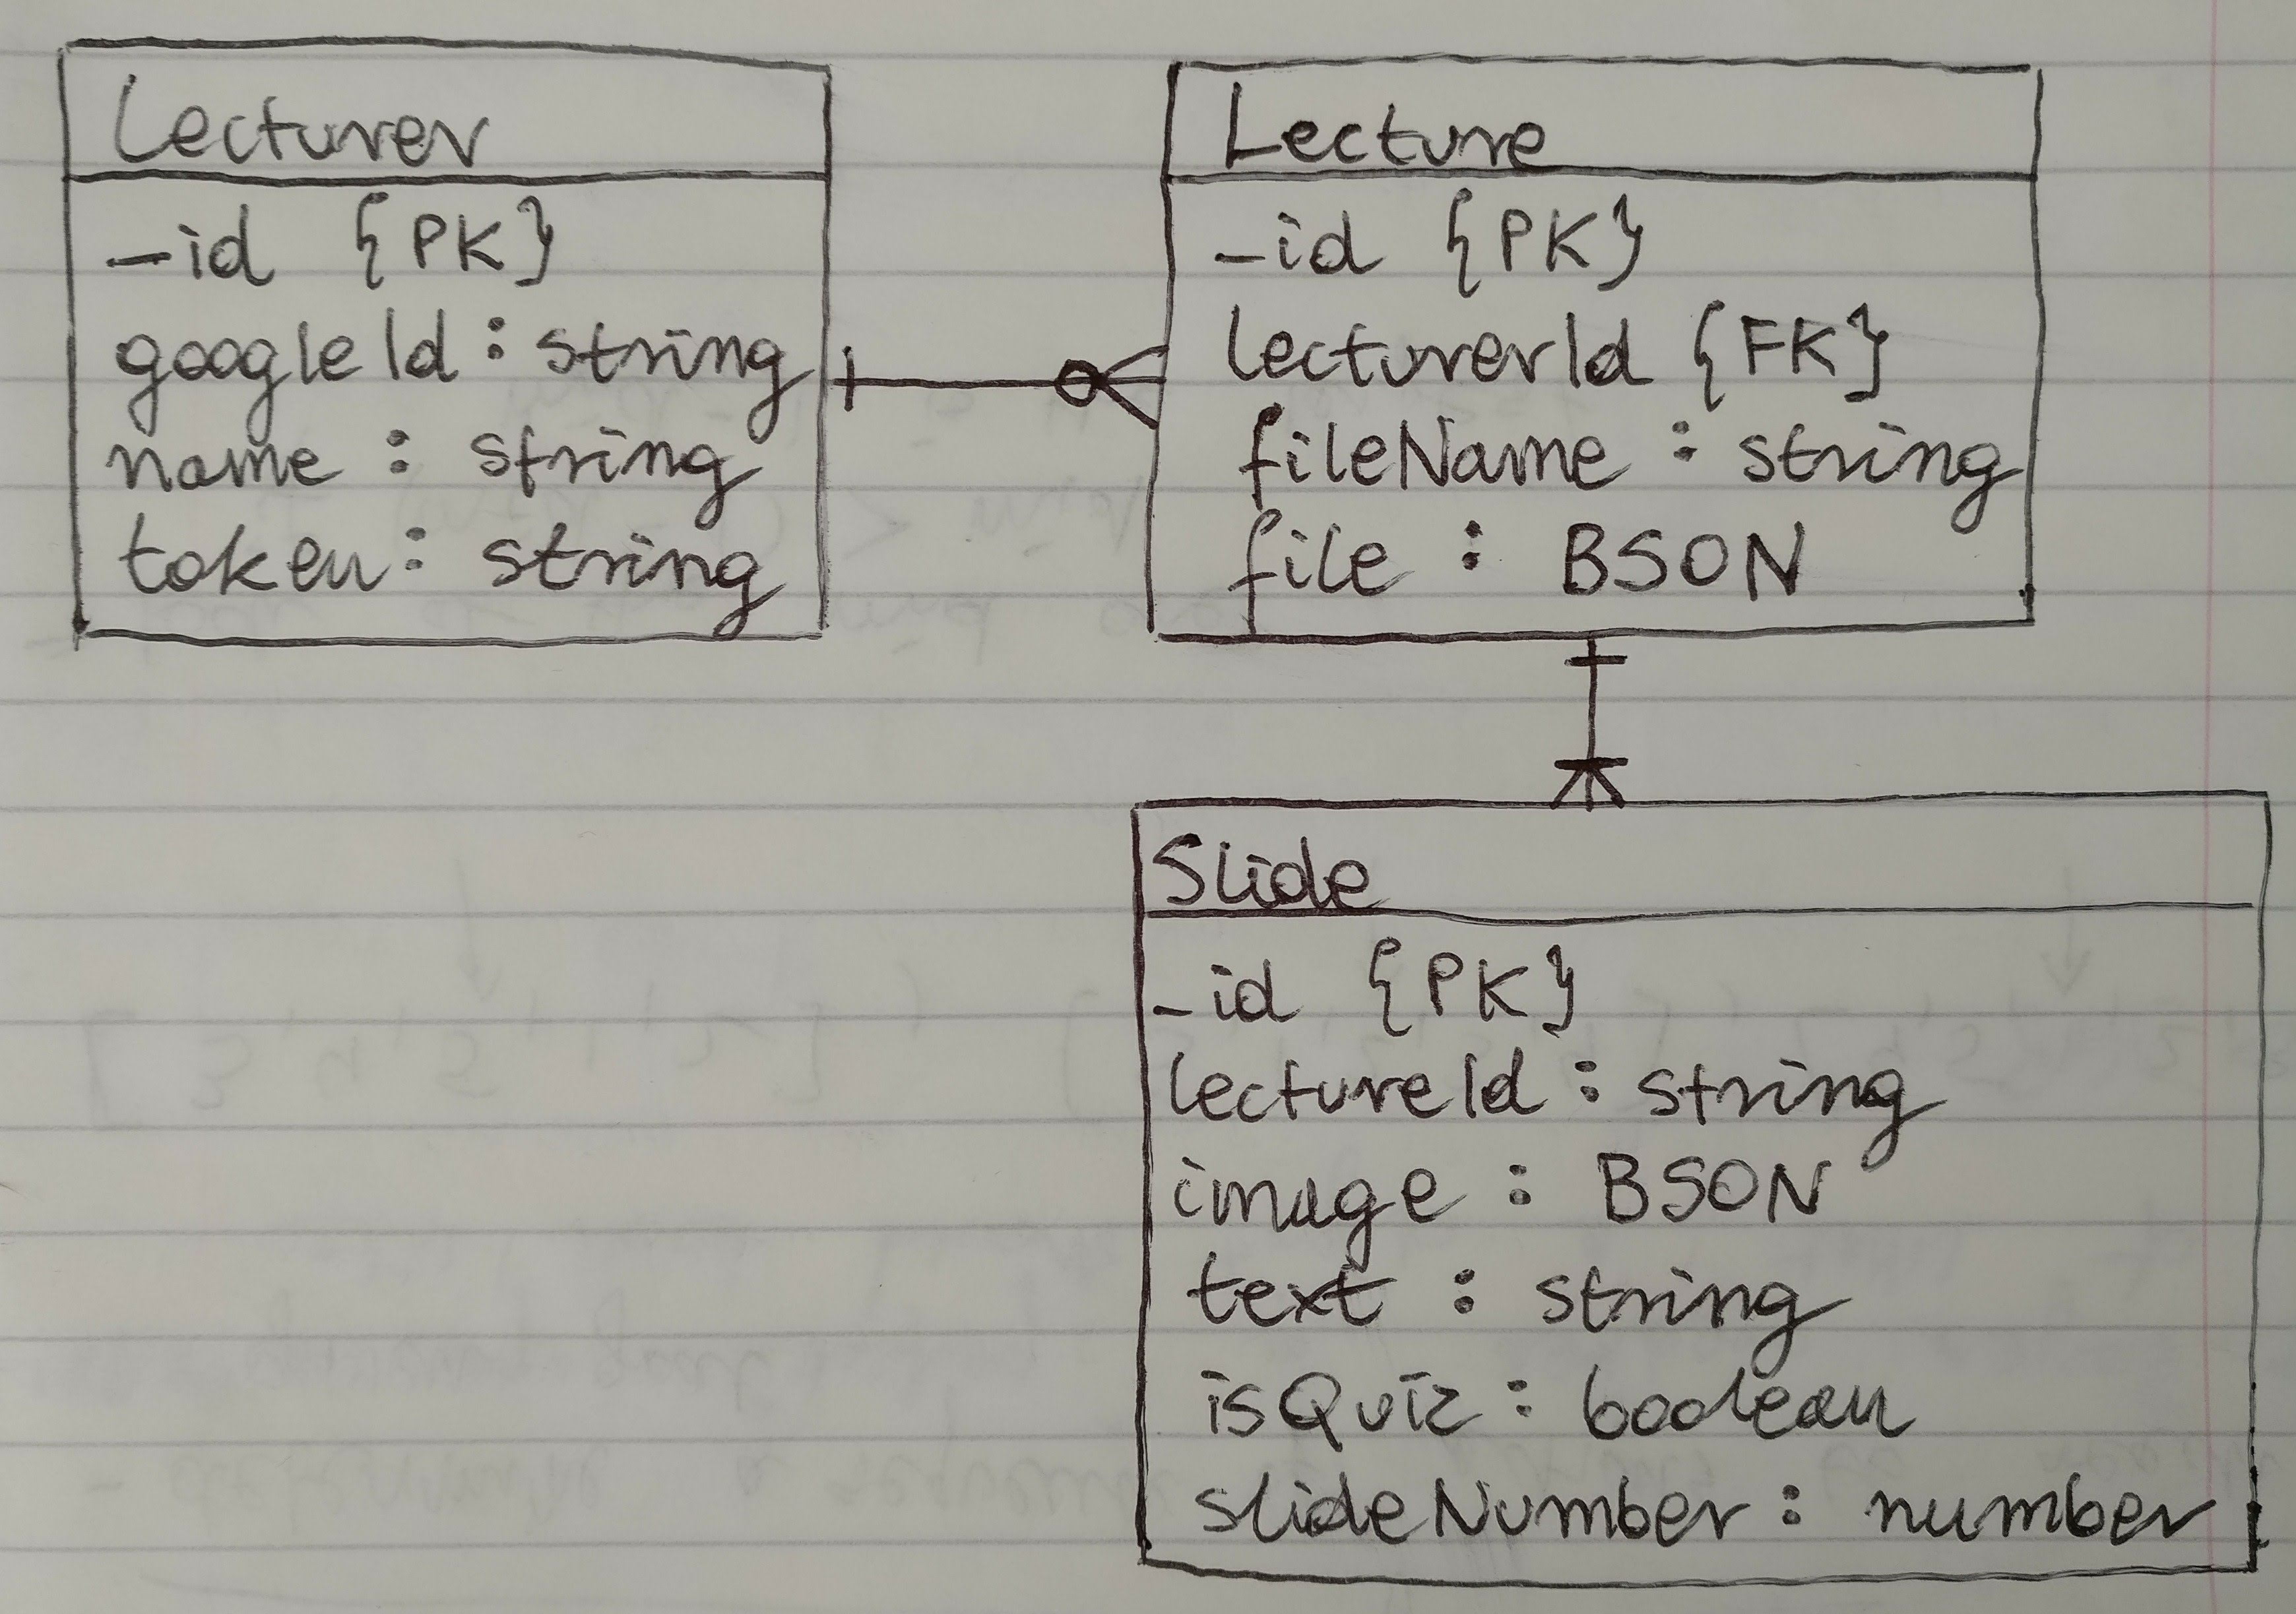
\includegraphics[width=0.8\textwidth]{initialERD.jpg}
    \caption{Initial Entity Relationship Diagram}
    \label{fig:initialERD}
\end{figure}

\subsection{Lecture Upload}

\begin{figure}[h!]
    \centering
    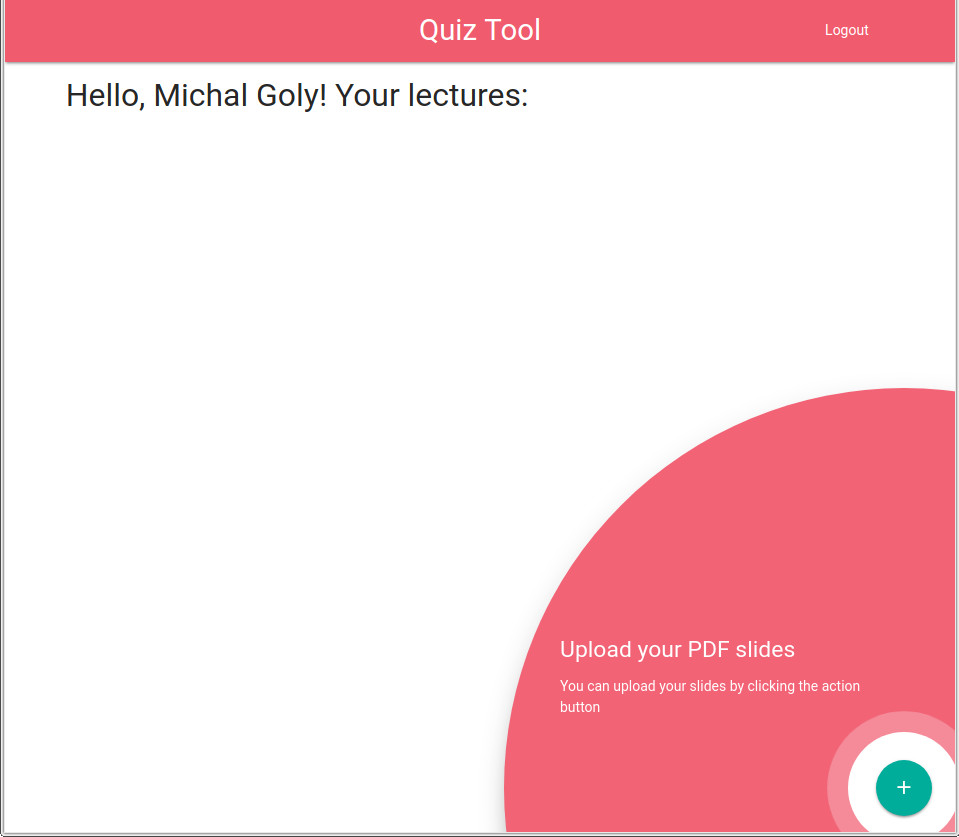
\includegraphics[width=0.8\textwidth]{dashboard.jpg}
    \caption{Dashboard View}
    \label{fig:dashboard}
\end{figure}

Once lecturer logs into the system he is presented with a dashboard view visible in the \autoref{fig:dashboard}.
The action button in the bottom right corner of the screen, allows PDF lecture slides to be uploaded.
The tool does not work with other presentation file formats for simplicity reasons. This could however
be extended in the future. Binary files can be stored in three major ways in MongoDB:

\begin{enumerate}
  \item Using the Mongoose BSON (Binary JSON)\cite{49} data type and setting it as type of a property of the document.
    This limits the file size to 16 MB.
  \item Using GridFS\cite{50} which relies on the client to have a driver capable of splitting the data into 255 KB
    chunks, and then streaming them into the database. This allows a binary file of any size to be persisted
    in MongoDB.
  \item Storing a file on an external storage, and persisting the reference to the file in the database.
\end{enumerate}

The BSON approach has been chosen for Quiz Tool, as it significantly simplified the implementation and it is
unlikely PDF presentations over 16 MB would be commonly used. Again, this is something that could be changed
in the future if the lifespan of the tool extended beyond the final project submission.

\begin{figure}[h!]
    \centering
    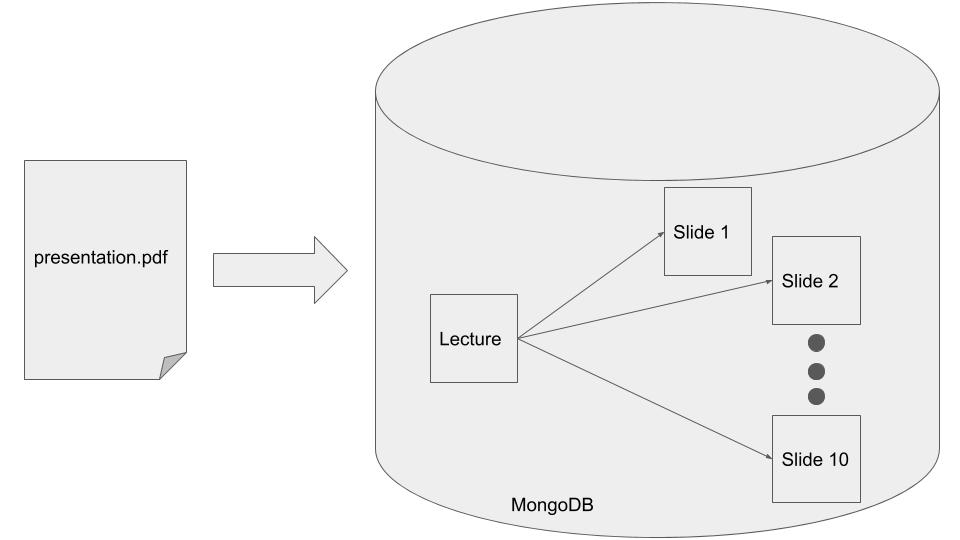
\includegraphics[width=0.8\textwidth]{fileupload.jpg}
    \caption{Initial File Upload}
    \label{fig:initialfileupload}
\end{figure}

The initial implementation of the file upload, took the PDF file, stored it directly as BSON in the
\texttt{Lecture} schema object and split the lecture into slides storing them in MongoDB using
the \texttt{Slide} schema object. Once the file has been uploaded using the ng2-file-upload\cite{51},
and persisted in the database, it has been stored temporarly on disk. Text would be extracted from
each slide using the pdf-extract\cite{52} library, which would be instructed to leave single paged
PDFs for each slide on disk. These PDFs would be then converted to PNG images using the scissors\cite{53}
library. Finally, slides' text and images would be grouped together and stored in MongoDB, before the
temporary files would be cleaned from disk.

\newpage
\subsection{Lecture Broadcast}

\subsection{Sprint Retrospective}


\section{Sprint 3 - Add Quizes}
\subsection{Sprint Planning}
This iteration focused on the ability to create quizzes, embed them into slides and
broadcast only to people who have the appropriate session key. The entire list of estimated stories
can be found in the \autoref{chap:spintstories} of this report.

\subsection{Sprint Retrospective}


\section{Sprint 4 - Fancy Quizes and Defect Fixing}
\subsection{Sprint Planning}
This sprint focused on addressing a critial bug in the production environment
concerning the PDF to PNG conversion. Extra types of quizzes would also be added
to complement the single choice ones availble at the moment. The entire list of estimated stories
can be found in the \autoref{chap:spintstories} of this report.

\subsection{Sprint Retrospective}
\section{Sprint 5 - Persistence, Report Generation and Testing}
\subsection{Sprint Planning}
The final sprint focused on the persistence of students' answers in the database and
generation of PDF reports based on these answers. User friendly error handler has
also been added, and the application has been polished before the Quiz Tool implementation
was over. As always, the entire list of estimated stories
can be found in the \autoref{chap:spintstories} of this report.

\subsection{Sprint Retrospective}

\chapter{Final Design}

This chapter follows on the discussion of the individual sprints and summarises
the final design of the tool.

\chapter{Testing}

\section{Server Side Unit Tests}
\section{Client Side Unit Tests}
\section{Selenium Integration Tests}

% You should concentrate on the more important aspects of the design. It is essential that an overview is presented before going into detail. As well as describing the design adopted it must also explain what other designs were considered and why they were rejected.
%
% The design should describe what you expected to do, and might also explain areas that you had to revise after some investigation.
%
% Typically, for an object-oriented design, the discussion will focus on the choice of objects and classes and the allocation of methods to classes. The use made of reusable components should be described and their source referenced. Particularly important decisions concerning data structures usually affect the architecture of a system and so should be described here.
%
% How much material you include on detailed design and implementation will depend very much on the nature of the project. It should not be padded out. Think about the significant aspects of your system. For example, describe the design of the user interface if it is a critical aspect of your system, or provide detail about methods and data structures that are not trivial. Do not spend time on long lists of trivial items and repetitive descriptions. If in doubt about what is appropriate, speak to your supervisor.
%
% You should also identify any support tools that you used. You should discuss your choice of implementation tools - programming language, compilers, database management system, program development environment, etc.
%
% Some example sub-sections may be as follows, but the specific sections are for you to define.

% \section{Overall Architecture}
%
% \section{Some detailed design}
%
% \subsection{Even more detail}
%
% \section{User Interface}
%
% \section{Other relevant sections}

% \chapter{Implementation}
% The implementation should look at any issues you encountered as you tried to implement your
% design. During the work, you might have found that elements of your design were unnecessary or
% overly complex; perhaps third party libraries were available that simplified some of the functions
% that you intended to implement. If things were easier in some areas, then how did you adapt your
% project to take account of your findings?
% It is more likely that things were more complex than you first thought. In particular, were there
% any problems or difficulties that you found during implementation that you had to address? Did
% such problems simply delay you or were they more significant?
% You can conclude this section by reviewing the end of the implementation stage against the
% planned requirements

% \chapter{Testing}
%
% Detailed descriptions of every test case are definitely not what is required here. What is important is to show that you adopted a sensible strategy that was, in principle, capable of testing the system adequately even if you did not have the time to test the system fully.
%
% Provide information in the body of your report and the appendix to explain the testing that has been performed. How does this testing address the requirements and design for the project?
%
% How comprehensive is the testing within the constraints of the project?  Are you testing the normal working behaviour? Are you testing the exceptional behaviour, e.g. error conditions? Are you testing security issues if they are relevant for your project?
%
% Have you tested your system on ``real users''? For example, if your system is supposed to solve a problem for a business, then it would be appropriate to present your approach to involve the users in the testing process and to record the results that you obtained. Depending on the level of detail, it is likely that you would put any detailed results in an appendix.
%
% The following sections indicate some areas you might include. Other sections may be more appropriate to your project.

% \section{Overall Approach to Testing}
%
% \section{Automated Testing}
%
% \subsection{Unit Tests}
%
% \subsection{User Interface Testing}
%
% \subsection{Stress Testing}
%
% \subsection{Other types of testing}
%
% \section{Integration Testing}
%
% \section{User Testing}
